\documentclass[a4paper]{article}
\usepackage[utf8]{inputenc}
\usepackage{amsmath}
\usepackage{siunitx}
\usepackage[ngerman]{babel}
\usepackage{pgfplots}
\usepackage{hyperref}
\usepackage{pgfplotstable}
\usepackage[section]{placeins}
\usepackage{enumitem}
\usepackage{float}
\usepackage{booktabs}
\usepackage[normalem]{ulem}
\usepackage{subcaption}

\pgfplotsset{compat=1.15}

% Full Reference, produces: "Abbildung 3: Schaltplan"
\newcommand*{\fullref}[1]{\hyperref[{#1}]{\autoref*{#1}: \nameref*{#1}}}

\title{GPET\\ Auswertung Versuch 6\\ Gruppe 1}

\author{Jonas Otto\\ \href{mailto:jonas@jonasotto.com}{jonas@jonasotto.com} 
   \and Luca Krüger \\ \href{mailto:luca.krueger@uni-ulm.de}{luca.krueger@uni-ulm.de} }
\date{vom   22. Mai 2018}

\begin{document}
    
\maketitle
\newpage
\section{Versuchsauswertung}

\subsection{Bestimmung der Grenzfrequenz}

Eine Messung der Bauteilgrößen von Kondensator und Widerstand mit dem Multimeter ergab die exakten Werte
\begin{equation*}
    \begin{split}
    R &= 0.996\si{k\ohm}\\
    C &= 2.11\si{\micro F}
\end{split}
\end{equation*}

Daraufhin wurde mit dem Oszilloskop die Grenzfrequenz gemessen (Abbildung \ref{fig:1-2-grenzfrequenz}), indem die Phasenverschiebeung gemessen wurde, die bei Grenzfrequenz genau $\varphi = \ang{45}$ betragen sollte. Der Frequenzgenerator wurde also so eingestellt, dass genau diese Phasenverschiebung erreicht wird. Dies war der Fall bei einer Grenzfrequenz von 
\begin{equation*}
    f_g=70.0\si{Hz}
\end{equation*}

\begin{figure}[H]
    \centering
    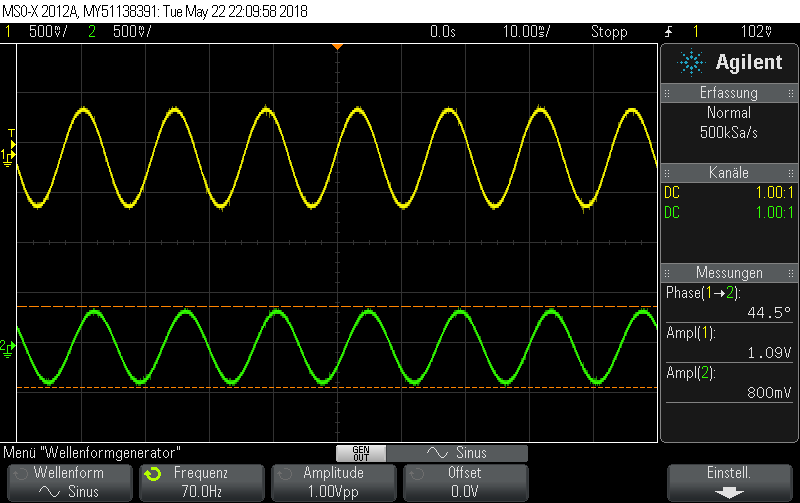
\includegraphics[width=0.8\textwidth]{versuch1/grenzfrequenz.png}
    \caption{Bestimmung der Grenzfrequenz}
    \label{fig:1-2-grenzfrequenz}
\end{figure}

Aus Gleichung 14 der Versuchsbeschreibung: $\varphi = -\arctan{(\frac{\omega R C}{1+ \frac{R}{R_L}})}$ und $\varphi = -\frac{\pi}{4} \implies \tan{(-\varphi)}=1$ bei $\omega = \omega_0$ ergibt sich der Innenwiderstand des Oszilloskops durch

%wobei \omega=2\pi*f nicht zu vergessen ist

\begin{equation*}
    R_i=\frac{R}{\omega R C - 1}=13.159\si{k\ohm}
\end{equation*}
Bei Abweichung der Frequenz von $1\%$ ergeben sich die Werte für den Innenwiderstand:
\begin{equation*}
    \begin{split}
        R_{i,f_g}     &= 13.159\si{\ohm}\\
        R_{i,f_g+1\%} &= 11.727\si{\ohm}\\
        R_{i,f_g-1\%} &= 14.99\si{k\ohm}
    \end{split}
\end{equation*}

Durch Messung mit dem Multimeter ergibt sich ein Innenwiderstand von
$R_i=0.998\si{M\ohm}$, laut Spezifikation liegt der Innenwiderstand des Oszilloskops bei $R_i=1\si{M\ohm}$.\\
Die gemessene Grenzfrequenz ist dem erwarteten Wert ähnlich. Für die Messung des Innenwiderstandes ist dieser Messaufbau allerdings viel zu ungenau. Deshalb weicht die Messung dort stark vom erwarteten Wert ab.

\subsection{Zeitverhalten eines Hochpasses}
Im folgenden Versuch wird das Sprungverhalten eines RC-Hochpasses erster Ordnung bei Anlegen einer Rechteckfunktion betrachtet.
Mit manueller Messung (Abbildung \ref{fig:2-manuell}) ergibt sich eine Falltime von
\begin{equation*}
    t_{\text{fall}} = 672\si{\micro s}
\end{equation*}
Bei Messung mit der eingebauten Messfunktion (Abbildung \ref{fig:2-measure}) ergibt sich eine Falltime von
\begin{equation*}
    t_{\text{fall}} = 666\si{\micro s}
\end{equation*}

\begin{figure}[H]
    \centering
    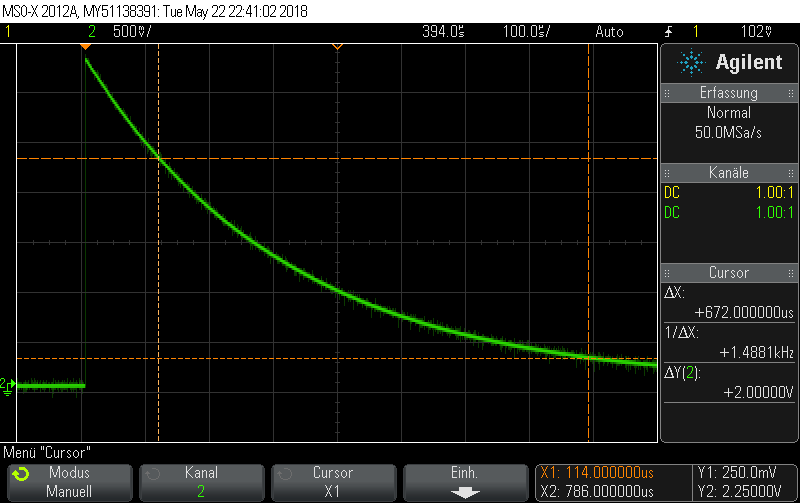
\includegraphics[width=0.8\textwidth]{versuch2/manuell.png}
    \caption{Manuelle Messung der Falltime}
    \label{fig:2-manuell}
\end{figure}

\begin{figure}[H]
    \centering
    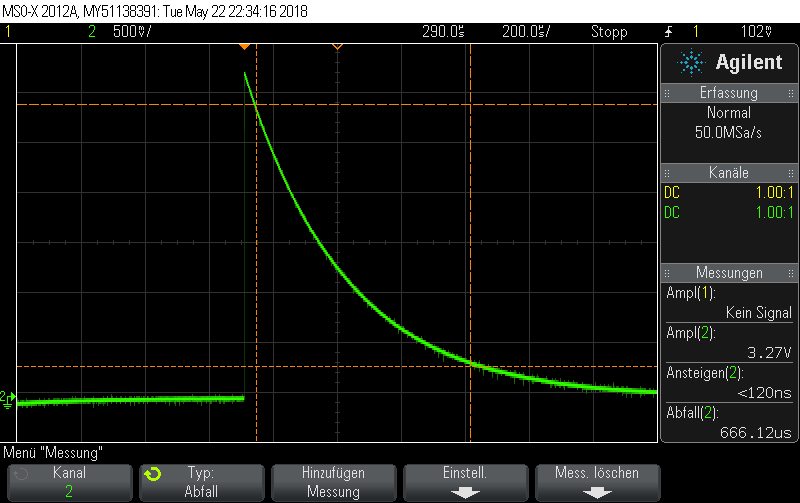
\includegraphics[width=0.8\textwidth]{versuch2/measure.png}
    \caption{Messung der Falltime mit Measure-Funktion}
    \label{fig:2-measure}
\end{figure}

\noindent Der theoretisch erwartete Wert für die Falltime beträgt
\begin{equation*}
    t_f=\tau \ln{(9)}=RC\ln{(9)}=483\si{\micro s}
\end{equation*}
Dies zeigt zwar eine große Abweichung zum Messwert, die Werte befinden sich aber in der gleichen Größenordnung. Die Abweichungen erklären sich durch Messfehler und Ungenauigkeiten der Bauteilgrößen. Außerdem zeigte das Oszilloskop einige Störungen auf dem Signal.

\subsection{Bandpass}
\label{subsec:versuch3-bandpass}
%TODO Übertragungsfkt Matlab: 100 Punkte, 1Vpp, 100Hz-100kHz, log
%TODO Diskutieren
Im folgenden wurde ein Bandpass erster Ordnung wie in Abbildung \ref{fig:versuch3-aufbau} betrachtet.
Das Diagramm entspricht der erwarteten Übertragungsfunktion des Bandpass-Filters. Der durchgelassene Bereich unter Beachtung der $3\si{dB}$-Grenzfrequenz liegt etwa bei $1\si{kHz}-10\si{kHz}$.

\begin{figure}[H]
    \centering
    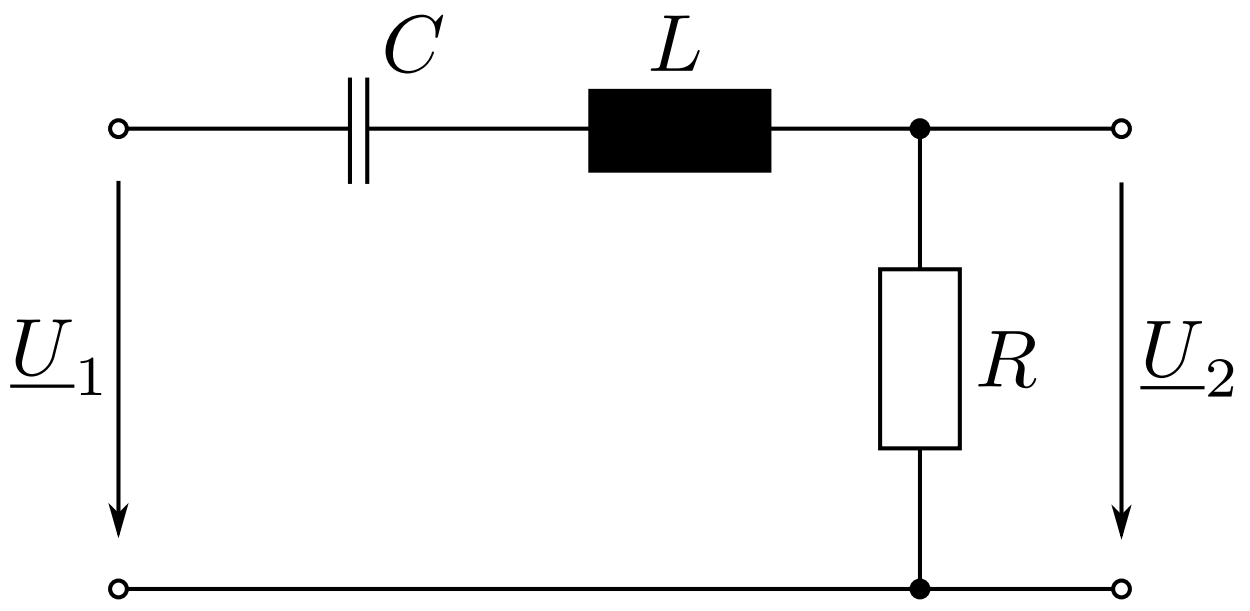
\includegraphics[width=0.8\textwidth]{versuch3/versuch3_aufbau.png}
    \caption{Versuchsaufbau zu Versuch: \nameref{subsec:versuch3-bandpass}}
    \label{fig:versuch3-aufbau}
\end{figure}

\begin{figure}[H]
    \centering
    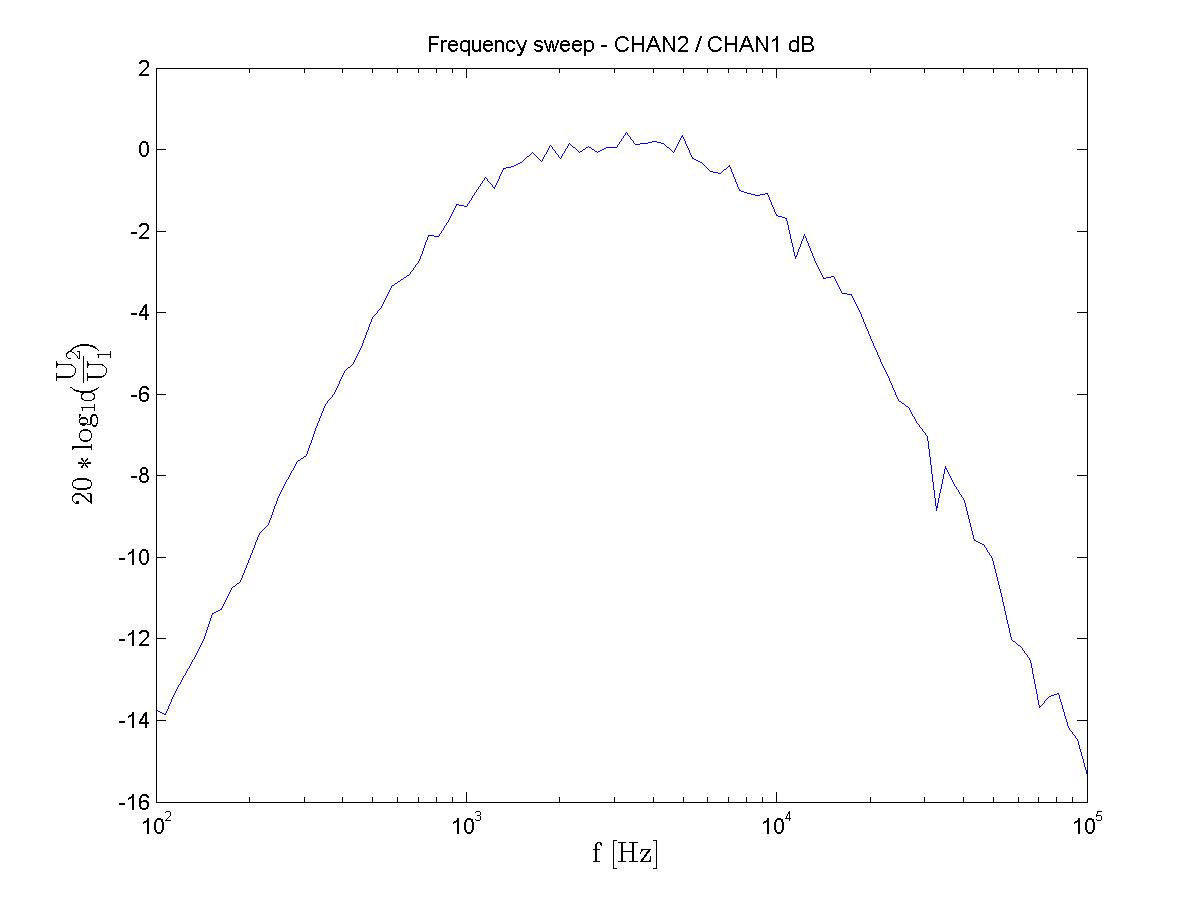
\includegraphics[width=0.8\textwidth]{versuch3/versuch3_uebertragungsfkt.jpg}
    \caption{Übertragungsfunktion Bandpass}
    \label{fig:versuch3-uebertragungsfkt}
\end{figure}

\subsection{Bandsperre}
\label{subsec:versuch4-bandsperre}
%TODO Übertragungsfkt Matlab: 100 Punkte, 1Vpp, 100Hz-100kHz, log
%TODO Diskutieren
In diesem Versuch wird eine Bandsperre (Abbildung \ref{fig:versuch4-aufbau}) betrachtet. Es wird erwartet dass nur ein bestimmtes Frequenzband gesperrt wird und die Dämpfung im restlichen Frequenzbereich gegen 0 geht.
Auch das Frequenzdiagramm der Bandsperre (Abbildung \ref{fig:versuch4-uebertragungsfkt}) entspricht den Erwartungen. Hier wird in etwa der gleiche Bereich, der im vorherigen Versuch durchgelassen wurde, nun gesperrt. Die Bandsperre liegt bei ($1\si{kHz}-10\si{kHz}$).

\begin{figure}[H]
    \centering
    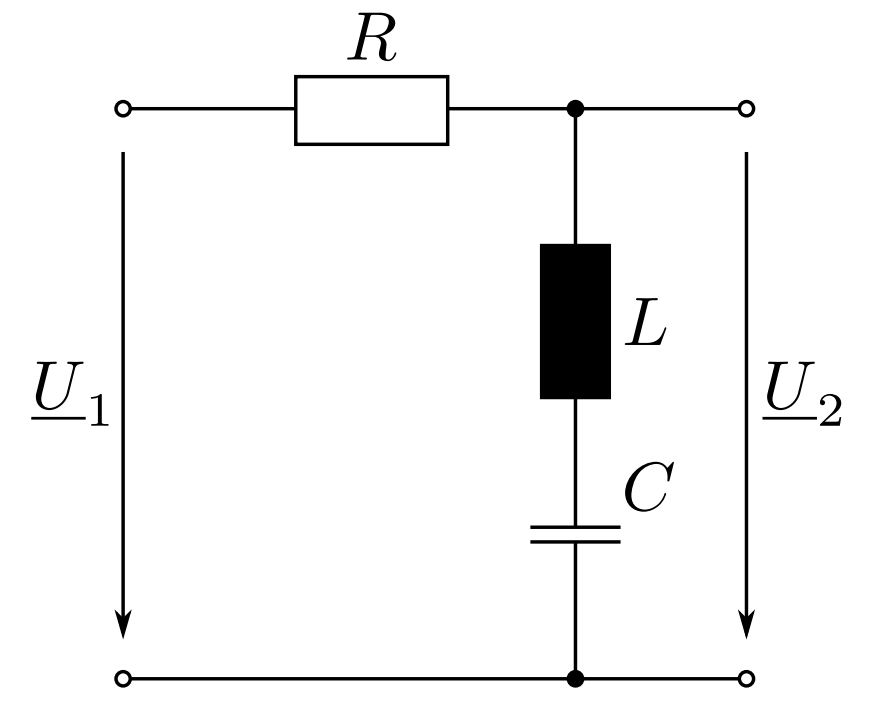
\includegraphics[width=0.8\textwidth]{versuch4/versuch4_aufbau.png}
    \caption{Versuchsaufbau zu Versuch: \nameref{subsec:versuch4-bandsperre}}
    \label{fig:versuch4-aufbau}
\end{figure}

\begin{figure}[H]
    \centering
    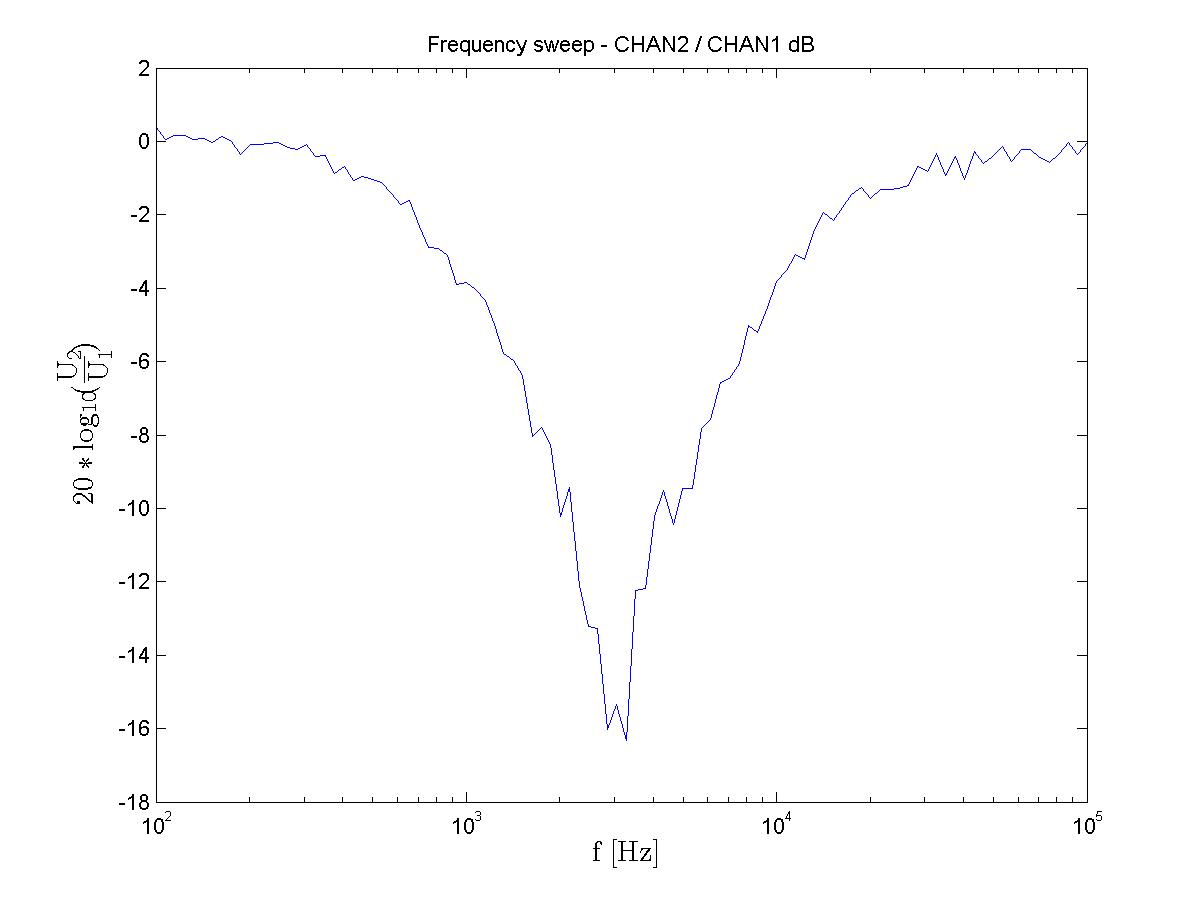
\includegraphics[width=0.8\textwidth]{versuch4/versuch4_uebertragungsfkt.jpg}
    \caption{Übertragungsfunktion Bandsperre}
    \label{fig:versuch4-uebertragungsfkt}
\end{figure}

\subsection{Frequenzbereich und Audio-Filterung}
\label{subsec:versuch5-audio}
In diesem Versuch war ein Audiosignal mit einer überlagerten Störung gegeben. Ziel war es die Störung zu identifizieren und das Störsignal mithilfe eines Hochpasses zu eliminieren.
Die Störung befindet sich im tiefen Frequenzbereich, vermutlich bei einer Frequenz $f<400\si{Hz}$.
%idk... 350hz?275?

\noindent Zunächst wurde der Widerstand des Kopfhörers gemessen, dieser beträgt $R=34.8\si{\ohm}$. Da die Plots einen Hochpass beschreiben, werden niedrige Frequenzen wie erwartet stark gedämpft, bei hohen Frequenzen geht die Dämpfung gegen $0\si{dB}$. Im unbelasteten Fall (Abbildung \ref{fig:versuch5-unbelastet}) wirkt der Filter bei Grenzfrequenz verstärkend (Resonanzfall). Dies verschwindet im belasteten Fall (Abbildung \ref{fig:versuch5-belastet}), da die entstehende Schwingung gedämpft wird.

\begin{figure}[H]
    \centering
    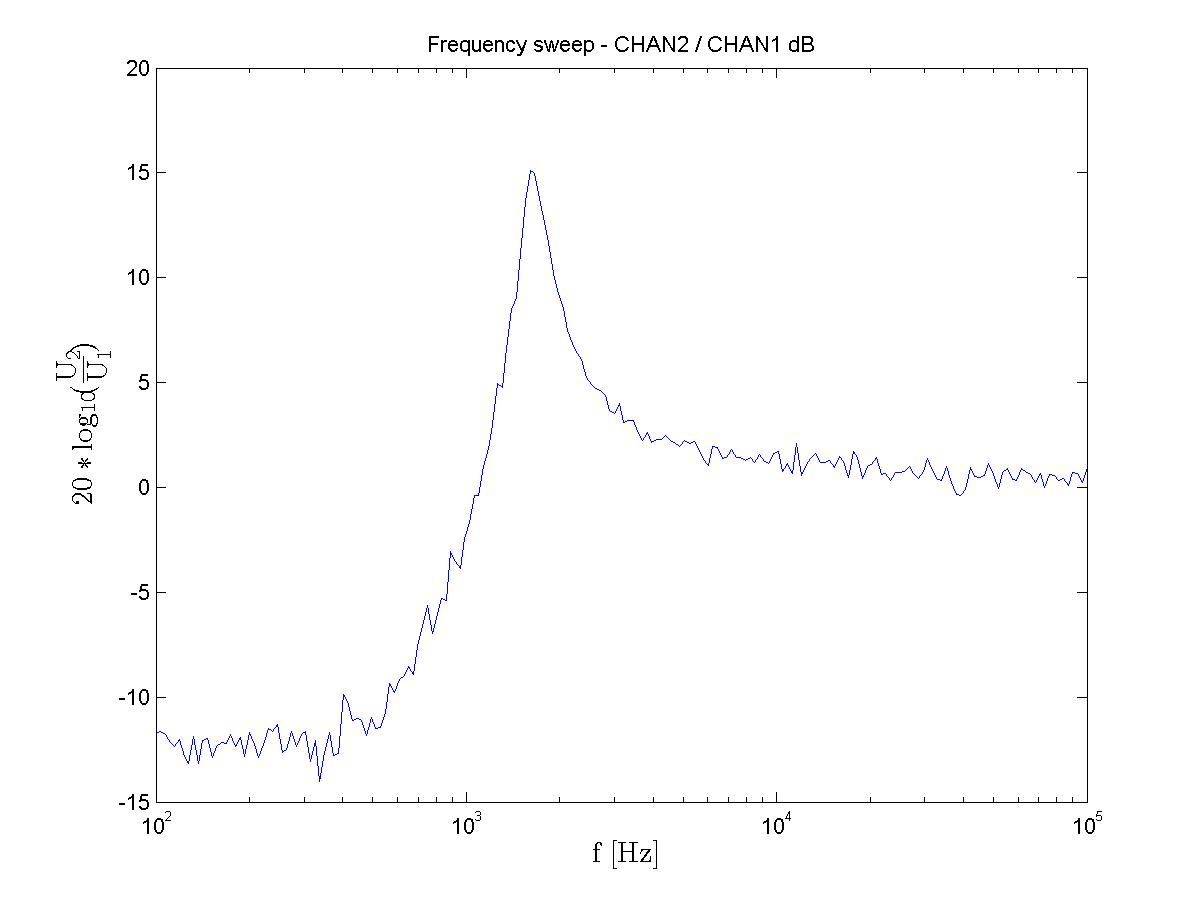
\includegraphics[width=0.8\textwidth]{versuch5/versuch5_unbelastet.jpg}
    \caption{Übertragungsfunktion des Hochpass-Filter (unbelastet)}
    \label{fig:versuch5-unbelastet}
\end{figure}

\begin{figure}[H]
    \centering
    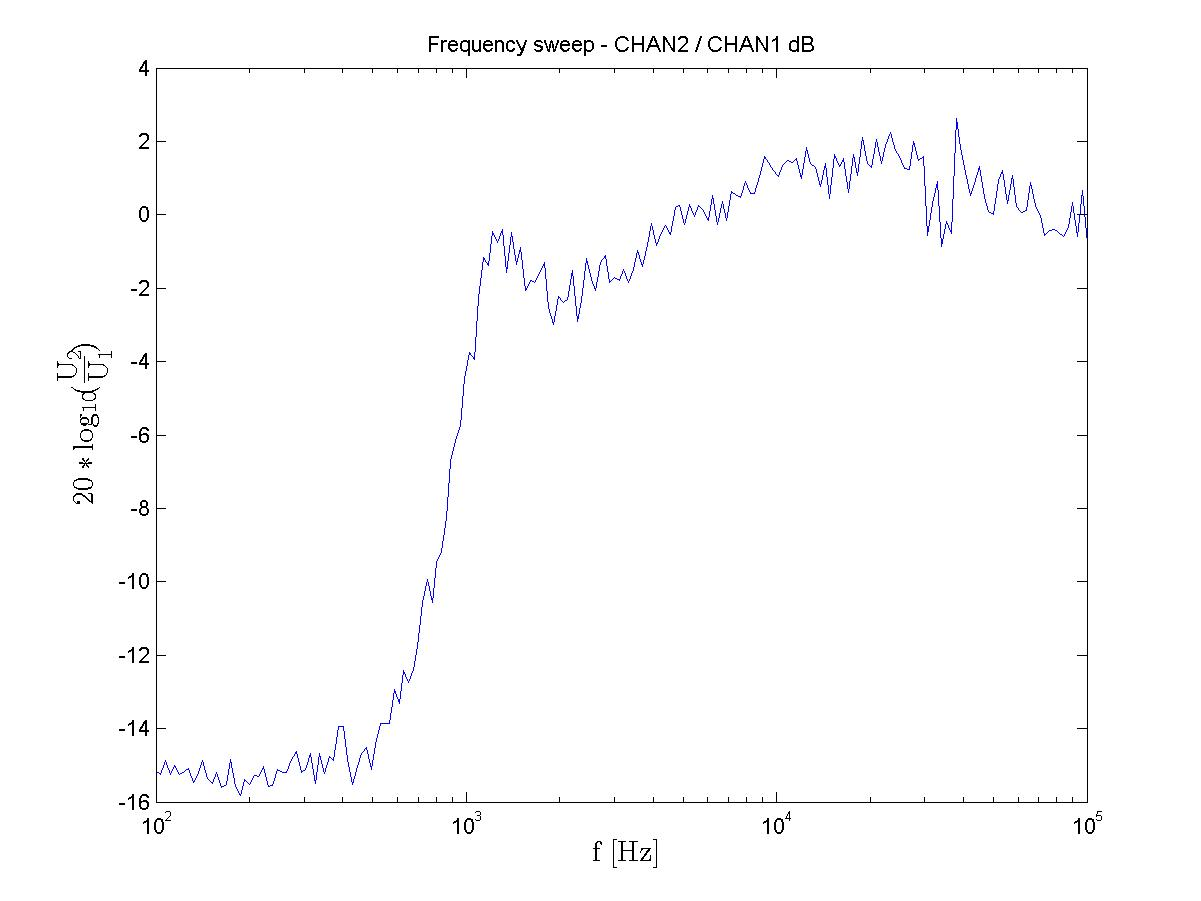
\includegraphics[width=0.8\textwidth]{versuch5/versuch5_belastet.jpg}
    \caption{Übertragungsfunktion des Hochpass-Filter (belastet)}
    \label{fig:versuch5-belastet}
\end{figure}

\noindent Leider kann man auch beim gefilterten Signal nicht erkennen welcher Satz gesprochen wurde. Der Sprecher könnte Donald Trump sein.
\end{document}